% Needs 2 passes, as the overlay is used!
\documentclass[margin=2pt]{standalone}
\usepackage[table]{xcolor}
\usepackage[utf8]{inputenc}
\usepackage[T1]{fontenc}

\usepackage{tikz}
\usepackage{helvet}
\usepackage{amsmath}
\usepackage{array}
\usepackage{tabularray}

\renewcommand\familydefault\sfdefault
\newcommand{\DisplayDirectory}{1}

\usetikzlibrary{intersections, shapes.arrows, spath3, shapes.geometric, fit, backgrounds, calc, tikzmark}

\definecolor{themeBlue}{RGB}{1, 103, 143}
\definecolor{themeOrange}{RGB}{221, 109, 16}
\definecolor{themeTeal}{RGB}{18, 54, 69}
\definecolor{themeGrey}{RGB}{120, 121, 124}

\begin{document}
    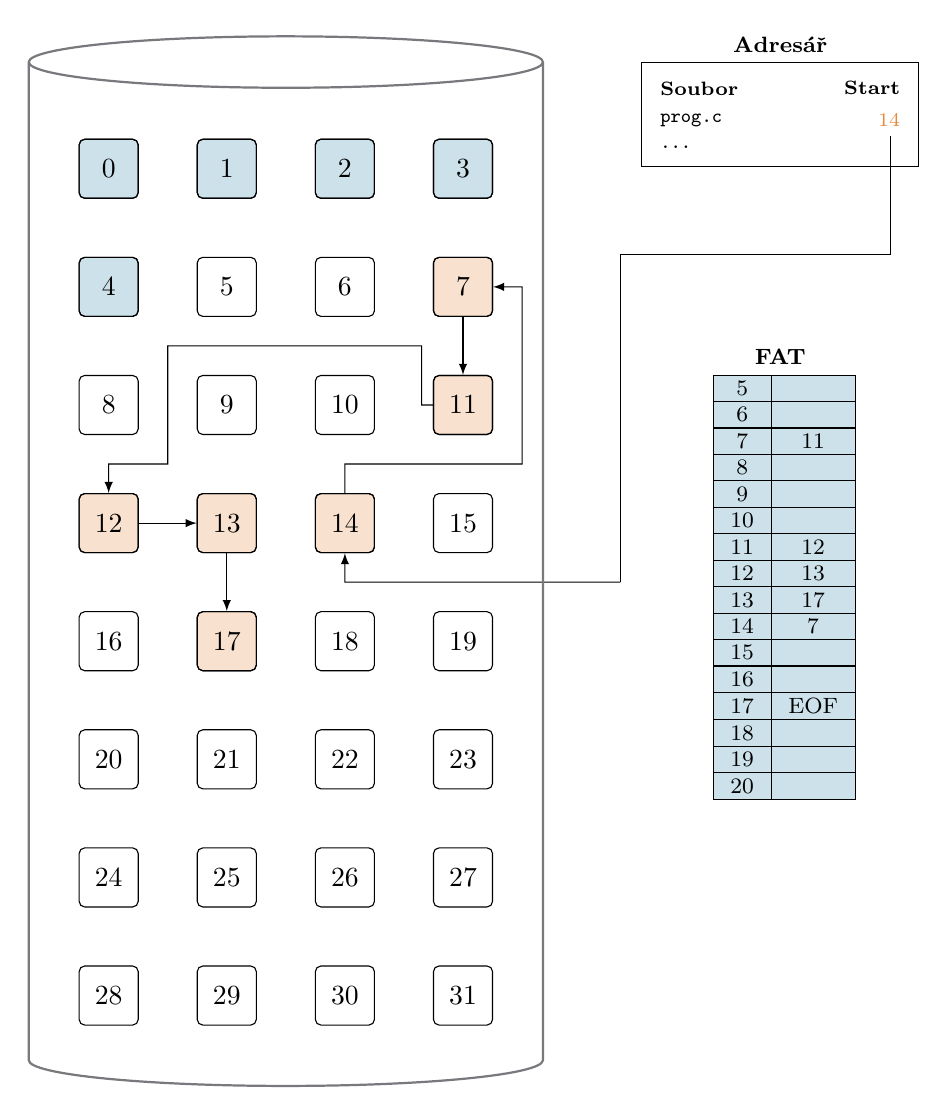
\begin{tikzpicture} [
        bus/.style={single arrow, single arrow head extend=2pt},
        hdd/.style={thick, cylinder, inner sep = 18pt, shape border rotate = 90, draw = themeGrey, aspect=0.1},
        cluster/.style={draw, minimum size=0.75cm, rounded corners=2pt},
        l/.style={align=left},
        r/.style={align=right},
        c/.style={align=center}
    ]
        \foreach \y in {0, ..., 7} {
            \foreach \x in {0, ..., 3} {
                \pgfmathtruncatemacro{\label}{\x + (\y * 4)}
               \node [cluster]  (\label) at (1.5*\x, -1.5*\y) {\label}; 
            }
        }
        \draw node[hdd, fit=(0) (31)] (c) {};
        
        \begin{scope}[on background layer]
            \foreach \n in {0, ..., 4} {
                \draw (\n) node [cluster, fill=themeBlue!20] {};
            }

            \foreach \n in {7, 11, 12, 13, 14, 17} {
                \draw (\n) node [cluster, fill=themeOrange!20] {};
            }

            \ifnum\DisplayDirectory=1
                \draw[latex-] (14.south) to ($ (\tikztostart)!.5!(\tikztostart|-18.north) $) -- ++(3.5, 0) coordinate (fs_in) node[] {\tikzmark{fs}};
    
                \draw[-latex] (14.north) 
                    to ($ (\tikztostart)!.5!(\tikztostart|-10.south) $)
                    to ($ (\tikztostart)!.4!(15|-\tikztostart) + (1.65,0) $) 
                    |- (7.east);
                %    to ();
                \draw[-latex] (7) -- (11);
                \draw[-latex] (11)
                    to ($ (10)!.65!(11) $)
                    to ($ (\tikztostart|-6)!.5!(\tikztostart|-10) $) 
                    to ($ (8|-\tikztostart)!.5!(9|-\tikztostart) $)
                    to ($ (\tikztostart|-13)!.5!(\tikztostart|-9) $)
                    -| (12);
                \draw[-latex] (12) -- (13);
                \draw[-latex] (13) -- (17);
            \fi
        \end{scope}
    
        \ifnum\DisplayDirectory=1
            \matrix (table) [draw, text width=4em, font=\scriptsize, anchor=north] at ($ (c.north east|-c.after top) +(3, 0) $) {
                \node[l] {\textbf{Soubor}};     & \node[r] {\textbf{Start}}; \\
                \node[l] {\texttt{prog.c}};     & \node[r] (f14) { \textcolor{themeOrange!80}{14} };      \\
                \node[l] {\texttt{\dots}};      & \node[r] { };        \\
            };
            \draw (table.north) node[above, anchor=south, font=\footnotesize] {\textbf{Adresář}};
            
            \draw (table) ++(0, -6) node[inner sep=0pt, font=\footnotesize] (fat) {
                \begingroup\setlength{\fboxsep}{0pt}
                \colorbox{themeBlue!20}{%
                \begin{tblr}{colspec={|Q[c,m]|Q[c,m]|}, stretch=0}%
                    \hline
                    5 &     \\ \hline
                    6  &     \\ \hline
                    7  & 11  \\ \hline
                    8  &     \\ \hline
                    9  &     \\ \hline
                    10 &     \\ \hline
                    11 & 12  \\ \hline
                    12 & 13  \\ \hline
                    13 & 17  \\ \hline
                    \tikzmark{fat}14 &  7  \\ \hline
                    15 &     \\ \hline
                    16 &     \\ \hline
                    17 & EOF \\ \hline
                    18 &     \\ \hline
                    19 &     \\ \hline
                    20 &     \\ \hline
                \end{tblr}%
                } \endgroup
            };

            \draw (fat.north) node[anchor=south, font=\footnotesize] {\textbf{FAT}};
            \draw (f14.south east) ++(-7pt, 0pt) to ++(0, -1.5) to (fs_in|-\tikztostart) to (fs_in);
        \fi
    \end{tikzpicture}
    
    \begin{tikzpicture}[overlay,remember picture]
        \ifnum\DisplayDirectory=1
            % Draw arrow to table
            \coordinate (t) at (pic cs:fat);
            \coordinate (f) at (pic cs:fs);
            \draw[latex-] (t) ++(-6pt, 2pt) coordinate (h) -- ++(-1,0) -- (f|-h) -- (f);
        \fi
    \end{tikzpicture}
\end{document}